\specialchapter{参考文献}

\begin{enumerate}
\def\labelenumi{\arabic{enumi}.}
\item
  L. EULER, 代数的完整教程 (=Opera Omnia (1), 第~I 卷，Leipzig-Berlin (Teubner)，1911).
\item
  J. L. LAGRANGE, 著作，14 卷，Paris (Gauthier-Villars)，1867--1892.
\item
  C. F. GAUSS, 著作，12 卷，Göttingen，1870--1927.
\item
  P. G. LEJEUNE-DIRICHLET, 著作，2 卷，Berlin (Reimer)，1889-1897.
\end{enumerate}

4 (bis). P. G. LEJEUNE-DIRICHLET, 数论讲义，第 2 版，Braunschweig (Vieweg)，1871.

\begin{enumerate}
\def\labelenumi{\arabic{enumi}.}
\setcounter{enumi}{4}
\item
  C. G. J. JACOBI, 著作集，7 卷，Berlin (Reimer)，1881-1891.
\item
  G. EISENSTEIN: (a) 关于由单位根的三次根组成的数的理论中三次剩余互反律的证明，Crelle's Journal，27 (1844)，第~289--310 页；(b) 关于素数 8n + 3、7n + 2 和 7n + 4 的二次分解理论，Crelle's Journal，37 (1848)，第~97--126 页；(c) 关于决定整个双纽线分割的方程的一些一般性质及其在数论中的应用，Crelle's Journal，39 (1850)，第~160--179 页和 224--287 页。
\item
  E. KUMMER: (a) 关于由实整数和单位根组成的复数，J. de Math.，(1)，12 (1847)，第~185--212 页；(b) 关于复数理论，Crelle's Journal，35 (1847)，第~319--326 页；(c) 关于由单位根构成的复数分解为素因子，Crelle's Journal，35 (1847)，第~327--367 页；(d) 关于由单位根和整数构成的复数的论文，J. de Math.，(1)，16 (1851)，第~377--498 页；(e) 关于次数为素数的幂的剩余与非剩余之间的一般互反律 (Abh. der Kön. Akad. der Wiss. zu Berlin (1859)，Math. Abhandl.，第~19--159 页)。
\item
  C. HERMITE, 著作，4 卷，Paris (Gauthier-Villars)，1905--1917.
\item
  L. KRONECKER, 著作，5 卷，Leipzig (Teubner)，1895--1930: (a) 关于复单位，第~I 卷，第~5--71 页 (=Inaug. Diss., Berolini，1845); (b) 关于代数可解方程 I，第~IV 卷，第~1--11 页 (=Monatsber. der Kön. Preuss. Akad. der Wiss.，1853，第~365--374 页); (c) 关于具有复乘法的椭圆函数，第~IV 卷，第~177--183 页 (=Monatsber. der Kön. Preuss. Akad. der Wiss.，1857，第~455--460 页); (d) 关于椭圆函数的复乘法，第~IV 卷，第~207--217 页 (=Monatsber. der Kön. Preuss. Akad. der Wiss.，1862，第~363--372 页); (e) 关于一个变量的代数函数的判别式，第~II 卷，第~193--236 页 (=Crelle's Journal，91 (1881)，第~301--334 页); (f) 代数数量的
\end{enumerate}

算术理论概要，第~II 卷，第~237--387 页 (=Crelle's Journal，92 (1882)，第~1--122 页)。

\begin{enumerate}
\def\labelenumi{\arabic{enumi}.}
\setcounter{enumi}{9}
\tightlist
\item
  R. DEDEKIND, 数学著作集，3 卷，Braunschweig (Vieweg)，1932: (a) 关于实素数模的高次同余理论概要，第~I 卷，第~40--66 页 (=Crelle's Journal，54 (1857)，第~1--26 页；(b) 关于代数整数理论，第~III 卷，第~262--296 页 (=Bull. Sci. Math.，(1)，11 (1876)，第~278--288 页和 (2)，1 (1877)，第~17--41 页、69--92 页、144--164 页、207--248 页); (c) 关于有限域不同阶中的理想类数，第~I 卷，第~105--157 页 (=Festschrift der Technischen Hochschule in Braunschweig zur Säkularfeier des Geburtstages von C. F. Gauss，Braunschweig，1877，第~1--55 页); (d) 关于理想理论与高次同余理论之间的联系，第~I 卷，第~202--230 页 (=Abh. Kön. Ges. Wiss. zu Göttingen，23 (1878)，第~1--23 页); (e) 关于有限域的判别式，第~I 卷，第~351--396 页 (=Abh. Kön. Ges. Wiss. zu Göttingen，29 (1882)，第~1--56 页); (f) 关于整代数数理论，第~III 卷，第~1--222 页 (=Supplement XI von Dirichlets Vorlesungen über Zahlentheorie，4 Aufl. (1894)，第~434--657 页); (g) 关于理想理论，第~II 卷，第~43--48 页 (=Nachr. Göttingen，1894，第~272--277 页); (h) 关于模理论中符号 (a, b) 的扩展，第~II 卷，第~59--85 页 (=Nachr. Göttingen，1895，第~183--208 页)。
\end{enumerate}

10 (bis). R. DEDEKIND-H. WEBER, 一个变量的代数函数理论，Crelle's Journal，92 (1882)，第~181--290 页 (=R. Dedekind, Ges. Math. Werke，第~I 卷，第~238--349 页)。

\begin{enumerate}
\def\labelenumi{\arabic{enumi}.}
\setcounter{enumi}{10}
\item
  E. SELLING, 关于由任意不可约方程的根有理构成的复数的理想素因子，Zeitschr. für Math. und Phys.，10 (1865)，第~17--47 页。
\item
  M. NOETHER, 关于代数函数理论中的一个定理，Math. Ann.，6 (1873)，第~351--359 页。
\item
  A. BRILL-M. NOETHER, 关于代数函数，Math. Ann.，7 (1874)，第~269--310 页。
\item
  G. ZOLOTAREFF, 关于复数理论，J. de Math. (3)，6 (1880)，第~51--84 页和 129--166 页。
\item
  E. NETTO, 关于消元理论，Acta Math.，7 (1885)，第~101-104 页。
\item
  D. HILBERT: (a) 关于代数型理论，Math. Ann.，36 (1890)，第~473--534 页；(b) 关于完备不变式系，Math. Ann.，42 (1893)，第~313--373 页；(c) Galois 数域理论概要，Gött. Nachr.，(1894)，第~224--236 页；(d) 数论报告，Jahresber. der D. M. V.，4 (1897)，第~175--546 页（由 A. Lévy 和 Th. Got 译成法文，题为 ``代数数域理论''，Paris (Hermann)，1913）。
\item
  K. WEIERSTRASS, 数学著作，7 卷，Berlin (Mayer und Müller)，1894--1927。
\item
  K. HENSEL: (a) 关于代数数理论的新基础，Jahresber. der D. M. V.，6 (1899)，第~83--88 页；(b) 关于代数域的基本方程与非本质判别因子，Gött. Nachr.，(1897)，第~254--260 页；(c) 算术的新基础，Crelle's Journal，127 (1902)，第~51--84 页；(d) 关于代数数和超越数的算术性质，Jahresber. der D. M. V.，14 (1905)，第~545--558 页；(e) 关于数的算术性质，Jahresber. der D. M. V.，16 (1907)，第~299--319 页、388--393 页、474--496 页；(f) 代数数理论，Leipzig (Teubner)，1908。
\item
  E. LASKER, 关于模与理想理论，Math. Ann.，60 (1905)，第~20--116 页。
\item
  E. STEINITZ: (a) 域的代数理论，Crelle's Journal，137 (1910)，第~167--308 页；(b) 代数数域中的矩形系统与模，Math. Ann. 71 (1912)，第~328--354 页和 72 (1912)，第~297--345 页。
\item
  F. S. MACAULAY, 关于给定模系统分解为准素系统，包括 Hilbert 数的某些性质，Math. Ann.，74 (1913)，第~66--121 页。
\item
  J. KÜRSCHAK, 关于极限构造与一般域理论，Crelle's Journal，142 (1913)，第~211--253 页。
\item
  A. FRAENKEL, 关于零因子与环的分解，Crelle's Journal，145 (1914)，第~139--176 页。
\item
  A. OSTROWSKI, 关于函数方程 \(\phi(x)\phi(y) = \phi(x.y)\) 的一些解，Acta Math.，41 (1917)，第~271-284 页。
\item
  E. NOETHER: (a) 环域中的理想理论，Math. Ann.，83 (1921)，第~24--66 页；(b) 代数数域和函数域中理想理论的抽象构造，Math. Ann.，96 (1927)，第~26--61 页。
\item
  H. HASSE: (a) 关于有理数域中用二次型表示数，Crelle's Journal，152 (1923)，第~129--148 页；(b) 关于有理数域中二次型的等价性，Crelle's Journal，152 (1923)，第~205--224 页；(c) Kurt Hensel 对发现局部--整体原理的决定性推动，Crelle's Journal，209 (1960)，第~3--4 页。
\item
  H. JUNG, 代数曲面，Hannover (Helwing)，1925。
\item
  H. GRELL, 不同环的理想之间的关系，Math. Ann.，97 (1927)，第~490-523 页。
\item
  W. KRULL: (a) 一般环域中的素理想链，Sitz. Ber. Heidelberg Akad. Wiss.，1928；(b) 一般赋值理论，Crelle's Journal，167 (1931)，第~160--196 页；(c) 交换整环算术的贡献，III，Math. Zeitschr.，42 (1937)，第~745--766 页；(d) 位环中的维数理论，Crelle's Journal，179 (1938)，第~204--226 页；(e) 理想理论，Berlin (Springer)，1935。
\item
  M. H. STONE: (a) 布尔代数的表示理论，Trans. Amer. Math. Soc.，40 (1936)，第~37-111 页；(b) 布尔环理论在一般拓扑中的应用，Trans. Amer. Math. Soc.，41 (1937)，第~375-481 页。
\item
  B. L. van der WAERDEN, 现代代数，第~II 卷，Berlin (Springer)，1931。
\item
  C. CHEVALLEY: (a) 无穷扩张的类域理论推广，J. de Math.，(9)，15 (1936)，第~359--371 页；(b) 局部环理论，Ann. of Math.，44 (1943)，第~690--708 页。
\item
  O. ZARISKI: (a) 抽象代数函数域的黎曼流形的紧性，Bull. Amer. Math. Soc.，50 (1944)，第~683--691 页；(b) 广义半局部环，Summa Bras. Math.，1 (1946)，第~169--195 页。
\item
  N. JACOBSON, 任意环的本原理想集上的拓扑，Proc. Nat. Acad. Sci. U.S.A.，31 (1945)，第~333--338 页。
\item
  I. COHEN-A.SEIDENBERG, 素理想与整独立性，Bull. Amer. Math. Soc.，52 (1946)，第~252--261 页。
\item
  P. SAMUEL, 代数与代数几何中的重数概念，J. de Math.，(9)，30 (1951)，第~159--274 页。
\item
  A. WEIL, 代数几何中的纤维空间（A. Wallace 笔记），Chicago Univ.，1952。
\item
  J. P. SERRE: (a) 凝聚代数层，Ann. of Math.，61 (1955)，第~197--278 页；(b) 代数几何与解析几何，Ann. Inst. Fourier，6 (1956)，第~1--42 页。
\item
  A. GROTHENDIECK, 代数几何原理，Publ. math. Inst. Htes Et. Scient.，1960。
\end{enumerate}

\specialchapter{记号索引}

参考编号依次表示章节、节和小节（或习题）。

\(l_{E}\)（E 为集合），U.V，UV（U、V 为加法子群），\(a^{0}\)（a 为理想）：第一章的预备约定

E:F:I.2.10

\(\mathbf{A}[\mathbf{S}^{-1}], a / s\)（A 为环，S 为 \(\mathbf{A}\) 的子集，\(a \in \mathbf{A}\)，\(s\) 为 \(\mathbf{S}\) 中元素的乘积）：II.2.1 \(i_{\mathbf{A}}^{\mathbf{S}}\) ：II.2.1

\(\mathbf{S}^{-1}\mathbf{A},\mathbf{A}_{p}\)（S 为乘性子集，p 为素理想）：II.2.1

\(\mathbf{M}[\mathbf{S}^{-1}], m / s, i_{\mathbf{M}}^{\mathbf{S}}\)（M 为 A-模，S 为 \(\mathbf{A}\) 的子集，\(m \in \mathbf{M}\)，\(s\) 为 \(\mathbf{S}\) 中元素的乘积）：II.2.2

\(S^{-1}M, M_{p}\)（M 为 A-模，S 为 A 的乘性子集，p 为 A 的素理想）：II.2.2

\(\mathbf{S}^{-1}u, u_{p}\)（\(u\) 为 A-模同态）：II.2.2

r(a)（a 为理想）：II.2.6

\(\mathbf{V}(\mathbf{M}), \mathbf{V}(f) (\mathbf{M}\) 是环 \(\mathbf{A}, f \in \mathbf{A})\)：II.4.3

\(\operatorname {Spec}(\mathbf{A})\) : II.4.3

\(\mathbf{X}_f\)（\(f \in \mathbf{A}\)，\(\mathbf{X} = \operatorname{Spec}(\mathbf{A})\)）：II.4.3

\(\Im (\mathbf{Y})\)（Y 是 \(\operatorname {Spec}(\mathbf{A}))\) 的子集）：II.4.3

\(^{a}h\)（h 为环同态）：II.4.3

Supp(M)（M 为 A-模）：II.4.4

\(\mathbf{A}_f, \mathbf{M}_f, u_f\)（A 为环，M 为 A-模，\(u\) 为 A-同态，\(f \in \mathbf{A}\)）：II.5.1

\(\mathbf{rg}_{\mathfrak{p}}(\mathbf{P})\)（P 为投射模）：II.5.3

rg(P)（P 为投射模）：II.5.3

\(P(A)\)，cl(M)（A 为环，M 为秩 1 的投射 A-模）：II.5.4

\(\operatorname{det}(u), \chi_u\)（\(u\) 为秩 \(n\) 的投射模的自同态）：II.5. 习题 9

\(\mathbf{A}^{(d)}, \mathbf{M}^{(d,k)}, \mathbf{M}^{(d)}\)（A 为分次环，M 为分次 A-模）：III.1.3

\(A_{(p)}, M_{(p)}\)（A 为分次环，p 为 A 的分次素理想，M 为分次 A-模）：III.1.4

\(\mathbf{gr}_n(\mathbf{G}), \mathbf{gr}(\mathbf{G})\)（G 为滤过群）：III.2.3

gr(h)（h 为与滤过相容的同态）：III.2.4

\(\mathbf{Z}_n\)（\(n\) 为整数 \(>1\)）：III.2.12

\(\hat{\mathbf{Z}}\) : III.2.13

\(\mathrm{A}\{\mathrm{X}_1,\dots ,\mathrm{X}_p\}\)（A 为线性拓扑环）：III.4.2

\(f(b_{1},\ldots ,b_{p})\)（f 为限制形式幂级数）：III.4.2

\(\mathbf{f} \circ \mathbf{g}, M_{t}, M_{t}(\mathbf{X}), J_{t}, J_{t}(\mathbf{X}), \mathbf{X}, \mathbf{1}_{n}\)（\(\mathbf{f}, \mathbf{g}\) 为形式幂级数系，\(\mathbf{g}\) 不含常数项）：III.4.4

\(\mathbf{f}(\mathbf{x})\)（f 为形式幂级数系，\(\mathbf{x}\) 为拓扑幂零元系）：III.4.5

\(\mathfrak{m}^{\times n}\)（m 为理想）：III.4.5

\(\operatorname{Ass}_{\mathbf{A}}(\mathbf{M}), \operatorname{Ass}(\mathbf{M})\)（M 为 A-模）：IV.1.1

\(\mathbf{Ass}_f(\mathbf{M})\) ：IV.1. 习题 17

\(\mathbf{A}^{\mathcal{G}}\)（A 为代数，\(\mathcal{G}\) 为作用在 A 上的群）：V.1.9

\(\mathcal{G}^{\mathrm{Z}}(\mathfrak{p}^{\prime}), \mathcal{G}^{\mathrm{Z}}, \mathrm{A}^{\mathrm{Z}}(\mathfrak{p}^{\prime}), \mathrm{A}^{\mathrm{Z}}\)（G 为作用在环 \(\mathrm{A}'\) 上的群，\(\mathfrak{p}'\) 为 \(\mathrm{A}'\) 的素理想）：V.2.2

\(\mathcal{G}^{\mathrm{T}}(\mathfrak{p}')\)，\(\mathcal{G}^{\mathrm{T}}\)，\(\mathbf{A}^{\mathrm{T}}(\mathfrak{p}')\)，\(\mathbf{A}^{\mathrm{T}}\)（\(\mathcal{G}\) 为作用在环 \(\mathbf{A}'\) 上的群，\(\mathfrak{p}'\) 为 \(\mathbf{A}'\) 的素理想）：V.2.2

\(\mathbf{K}^{\mathrm{Z}}(\mathfrak{p}')\)，\(\mathbf{K}^{\mathrm{Z}}\)，\(\mathbf{K}^{\mathrm{T}}(\mathfrak{p}')\)，\(\mathbf{K}^{\mathrm{T}}\)（K 是整闭整环

A 的分式域，\(p'\) 是 K 的拟 Galois 扩张中 A 的整闭包的素理想）：V.2.3

\(\mathbf{Y}^{\mathbf{p}}\)（其中 \(\mathbf{p} = (p_1, \ldots, p_m)\)，\(p_i\) 为整数 \(\geqslant 0\)）：V.3.1

\(\mathfrak{m}(\mathbf{A}), \kappa(\mathbf{A}), \mathrm{U}(\mathbf{A})\)（A 为局部环）：VI

\(\tilde{\mathbf{K}},\infty :\mathbf{VI}.2.1\)

+∞: VI.3.1

\(\Gamma_{\mathbf{A}}, v_{\mathbf{A}}\) : VI.3.2

\(\mathfrak{a}(\mathbf{M})\)（M 为优势集）：VI.3.5

\(h(\mathbf{G})\)（G 为全序群）：VI.4.4

\(\mathcal{T}_v\)（\(v\) 为赋值）：VI.5.2

\(e(v^{\prime} / v), e(\mathbf{A}^{\prime} / \mathbf{A}), e(\mathbf{L} / \mathbf{K})\) : VI.8.1

\(f(v^{\prime} / v),f(\mathbf{A}^{\prime} / \mathbf{A}),f(\mathbf{L} / \mathbf{K})\) : VI.8.1

\(\varepsilon (\mathrm{G},\mathrm{H})\)（G 为全序群，H 为 G 的有限指数子群）：VI.8.4

\(\varepsilon(v'/v)\)（\(v\) 为赋值，\(v'\) 为 \(v\) 的扩张）：VI.8.4

mod(x), mod\_K(x)（K 为非离散局部紧域，x ∈ K）：VI.9.1

\(r(\mathbf{G})\)（交换群的有理秩）：VI.10.2

\(d(\mathbf{K}' / \mathbf{K}), s(v' / v), r(v' / v)\)（v 为 \(\mathbf{K}\) 上的赋值，\(v'\) 为 \(v\) 在超越扩张 \(\mathbf{K}'\)（\(\mathbf{K}\) 的）上的扩张）：VI.10.3

I(A), D(A)（A 为整环）：VII.1.1

\(\mathfrak{a} \prec \mathfrak{b}\)，\(\operatorname{div}(\mathfrak{a})\)，\(\operatorname{div}(x)\)（\(\mathfrak{a}\)、\(\mathfrak{b}\) 为分式理想，\(x\) 为分式域的元素）：VII.1.1

\(\tilde{\mathfrak{a}}\)（a 为分式理想）：VII.1.1

\(d_{1} \leqslant d_{2}\)（\(d_{1}, d_{2}\) 为除子）：VII.1.1

b: a（a、b 为分式理想）：VII.1.1

J(A)（A 为整环）：VII.1.2

P(A)（A 为 Krull 整环）：VII.1.3

\(\mathfrak{p}^{(n)}\)（p 为除性素理想）：VII.1.4

\(v_{p}\)（p 为 Krull 整环中高度 1 的素理想）：VII.1.10

\(\mathbf{F}(\mathbf{A}), \mathbf{C}(\mathbf{A})\)（A 为 Krull 整环）：VII.1.10

\(e(\mathfrak{P}/\mathfrak{p})\) \((\mathfrak{p}\in\mathrm{P}(\mathrm{A}),\;\mathfrak{P}\in\mathrm{P}(\mathrm{B}),\;\mathrm{A}\;\text{和}\;\mathrm{B}\;\text{Krull 整环},\;\mathrm{A}\subset\mathrm{B},\;\mathfrak{P}\cap\mathrm{A}=\mathfrak{p}):\) VII.1.10

\(i\)（从 \(\mathbf{D}(\mathbf{A})\) 到 \(\mathbf{D}(\mathbf{B})\) 的同态，或从 \(\mathbf{C}(\mathbf{A})\) 到 \(\mathbf{C}(\mathbf{B}))\) 的同态）：VII.1.10

\(\bar{i}\)（从 \(\mathbf{C}(\mathbf{A})\) 到 \(\mathbf{C}(\mathbf{B}))\) 的同态）：VII.1.10

\(A, A_{0}, \Delta(K)\)（限制阿代尔的环）：VII.2.4

\(\mathfrak{P}^*, \mathfrak{P}^*(\mathbf{A})\)（A 为整环）：VII.3.2

M*（格 M 的对偶格）：VII.4.2

\(l_{\mathfrak{p}}(\mathrm{T}), \chi (\mathrm{T})\)（T 为扭 A-模，\(\mathfrak{p}\) 为高度 1 的素理想）：VII.4.5

\(\pmb {F}(\mathbf{A}),\pmb{T}(\mathbf{A}),\mathrm{cl}(\mathbf{M}):\) VII.4.5

\(\chi (\mathbf{M},\mathbf{M}^{\prime})\)（M、\(\mathbf{M}'\) 为格）：VII.4.6

\(c(d)\)（\(d\) 为除子）：VII.4.7

\(c(\mathbf{M}), r(\mathbf{M}), \gamma(\mathbf{M})\)（M 为格）：VII.4.7

\(\mathfrak{P}|\mathfrak{p},e_{\mathfrak{P} / \mathfrak{p}},f_{\mathfrak{P} / \mathfrak{p}},f(\mathfrak{P} / \mathfrak{p})\)（A \(\subset\) B 为 Krull 整环，且 B 是有限 A-代数

\(\mathfrak{p} \in \mathrm{P}(\mathbf{A}), \mathfrak{P} \in \mathrm{P}(\mathbf{B}), \mathfrak{P} \cap \mathbf{A} = \mathfrak{p}\) : VII.4.8

\(\mathbf{N}_{\mathbf{B} / \mathbf{A}},\mathbf{N},i_{\mathbf{B} / \mathbf{A}}\) :VII.4.8

\specialchapter{术语索引}

参考编号依次表示章节、节和小节（或习题）。

阿代尔、限制阿代尔、主限制阿代尔：VII.2.4

m-进滤过：III.2.1

--- 拓扑：III.2.5

\(n\)-进整数：III.2.12

Azumaya 代数：II.1.7

--- 有限生成的：III.1.1

--- 在环上整且有限的：V.1.1

域在代数中的代数闭包：V.1.2

在代数中代数闭的域：V.1.2

--- 代数相关、无关的元素：III.1.1

--- 代数自由、相关的族：III.1.1

对几乎所有 \(\mathfrak{p} \in \mathbf{P}(\mathbf{A})\)（成立的性质）：VII.4.3

--- 殆幂零自同态：IV.1.4

绝对值逼近定理：VI.7.3

--- 赋值逼近定理：VI.7.2

Artin-Rees 引理：III.3.1

与分次模相伴的（滤过模）：III.2.1

--- 与分次环相伴的（滤过环）：III.2.1

--- 与分次相伴的（滤过）：III.2.1

--- 与滤过相容的同态相伴的分次同态：III.2.4

--- 与滤过模相伴的（分次模）：III.2.3

--- 与滤过环相伴的（分次环）：III.2.3

--- 与环同态相伴的（映射）：II.4.3

--- 与模相伴的（素理想）：IV.1.1

--- 伴随环、位、赋值：VI.3.3

位的典范分解：VI.2.3

--- 赋值的典范分解：VI.3.2

--- 从素理想 \(\mathfrak{p}'\) 的分解群到

A'/p' 的自同构群的典范同态：V.2.2

与有限生成模相联的除子类：VII.4.7

除子类（除子幺半群）：VII.1.2

域在代数中的代数闭包：V.1.2

--- 整环的整闭包：V.1.2

--- 环在代数中的整闭包：V.1.2

交换图：I.1.2

（滤过）与环结构、模结构相容：III.2.1

--- （同态）与滤过相容：III.2.4

赋值扩张的完备系：VI.8.2

完全整闭整环：V.1.4

不可约分支（拓扑空间的）：II.4.1

Hensel 条件：III.4.5

子模的导子：V.1.5

伪 Bézout 整环上多项式的容度：VII.1.习题 23

--- 扭模的容度：VII.4.5

Eisenstein 不可约判别法：VII.3.习题 20

位的典范分解：VI.2.3

--- 素理想的完全分解：V.2.2

--- 素理想的分解域：V.2.2

--- 素理想的分解群、分解环：V.2.2

--- Dedekind 整环中理想分解为素因子：VII.2.3

--- 准素：IV.2.2 和习题 20

--- 既约准素：IV.2.3 和习题 20

递减滤过：III.2.1

Dedekind 整环：VII.2.1

（拓扑）由滤过定义：III.2.5

定义理想：III.3.2

一个赋值相对于另一个赋值的剩余类次数：VI.8.1

整依赖（方程）：V.1.1

（模滤过）由环滤过导出：III.2.1

交换图：I.1.2

--- 蛇形图：I.1.4

离散滤过：III.2.1

--- 离散赋值：VI.3.6

特异多项式：VII.3.8

除子、主除子：VII.1.1

--- 行列式除子：VII.4.习题 11

--- 有限生成除子：VII.1.习题 11

除性分式理想：VII.1.1

等价除子：VII.1.2

整环，Bézout（或 Bezout）：VII.1.习题 20

--- 完全整闭整环：V.1.4

--- Dedekind 整环：VII.2.1

--- 因子分解整环：VII.3.1

--- 整闭整环：V.1.2

--- 有限特征的整闭整环：VII.1.习题 25、26 和 28

--- 整 Noether 整环：V.3.习题 6

--- Krull 整环：VII.1.3

--- 一维局部整环：VI.4.习题 7

--- Prüfer 整环（或 Prüfer）：VII.2.习题 12

--- 伪 Bézout 整环：VII.1.习题 21

--- 伪主理想整环：VII.1.习题 21

--- 伪 Prüfer 整环：VII.2.习题 19

--- 正则整闭整环：VII.1.习题 30

支配（局部环）局部环：VI.1.1

模的代数托里克对偶：VI.5.习题 9

--- 格的对偶：VII.4.2

--- 拓扑托里克对偶：VI.5.习题 10

拓扑幂零元：III.4.3

代数相关、无关的元素：III.1.1

--- 强互素的元素：III.4.1

殆幂零自同态：IV.1.4

等价除子：VII.1.2

--- 等价赋值：VI.3.2

本性分次理想：III.1.4

--- 本性赋值：VII.1.4

欧氏有序域：VI.2.习题 4

穷竭滤过：III.2.1

拟 Galois 扩张：V.2.2

不变因子：VII.4.习题 11 和 14

因子分解整环：VII.3.1

赋值的典范分解：VI.3.2

忠实平坦模：I.3.1

代数自由、相关的族：III.1.1

--- 形式自由的：III.2.9

在代数中代数闭的域：V.1.2

--- 分解域：V.2.3

--- 射影域：VI.2.1

--- 局部环的剩余域：II.3.1

位的剩余域：VI.2.3

--- 赋值的剩余域：VI.3.2

--- 位的值域：VI.2.2

滤过群、环、模：III.2.1

m-进滤过：III.2.1

--- 与分次相伴的：III.2.1

--- 与环结构、模结构相容的：III.2.1

--- 离散的：III.2.5

--- m-好的：III.3.1

--- 递增、递减、分离、穷竭滤过：III.2.1

--- 诱导的、乘积的、商的：III.2.1

--- 由环滤过导出的模滤过：III.2.1

--- 平凡的：III.2

环上的有限代数：V.1.1

--- （位）在元素处有限：VI.2.2

有限生成代数：III.1.1

有限表示的：I.2.8

对 M 平坦、M-平坦（模）：I.2.2

--- 平坦模：I.2.3

形式自由族：III.2.9

分式理想：VII.1.1

阶函数：III.2.2

Gauss 整数：V.1.1

Gauss 引理：VII.3.5

Gelfand-Mazur 定理：VI.6.4.

由子集生成（乘性子集）：II.2.1

生成元的形式系：III.2.9

m-好滤过：III.3.1

分解群：V.2.2

--- 滤过群：III.2.1

--- 惯性群：V.2.2

--- 可逆模类群：II.5.7

--- 局部有限算子群：V.1.9

--- 作用在环上的群：V.1.9

--- 赋值的阶群：VI.3.2

--- 高度 n、高度 +∞ 的有序群：VI.4.4

高度 \(\leqslant 1\)（素理想的）：VII.1.6

--- 有序群、赋值的高：VI.4.4

Hensel 环：III.4.习题 3

Hensel 条件：III.4.5

--- 定理：III.4.3

素理想 \(p'\) 的分解群的典范同态

--- 从 A' 到 A'/p' 的自同构群：V.2.2

--- 与滤过相容：III.2.4

--- 与滤过相容的同态相伴的分次同态：III.2.4

--- 局部同态：II.3.1

--- 伪单射、伪满射、伪零、伪双射：VII.4.4

行列式理想：VII.4.习题 10 和 14

--- 本性分次理想：III.1.4

--- 浸入素理想：IV.2.3

--- 整理想、分式理想：VII.1.1

--- 可逆分式理想：II.5.7

--- 位于理想之上的理想：V.2.1

--- 极小素理想：II.2.6

--- 位的理想：VI.2.3

--- 赋值的理想：VI.3.2

--- 素理想：II.1.1

--- 与模相伴的素理想：IV.1.1

--- 完全分解的素理想：V.2.2

--- 高度 ≤1 的素理想：VII.1.6

--- 准素、p-准素理想：IV.2.1 和习题 20

--- 非分歧理想：V.2.习题 18 和 19

理想 Hausdorff 模：III.5.1

互素理想：II.1.2

Cauchy 恒等式：VII.3.习题 18

浸入素理想：IV.2.3

非真赋值：VI.3.1

递增滤过：III.2.1

独立赋值环：VI.7.2

--- 独立赋值：VI.7.2

有序群子群的初始指数、赋值的初始分歧指数：VI.8.4

--- 分歧指数：VI.8.1

诱导滤过：III.2.1

Noether 归纳法（原则）：II.4.2

惯性域：V.2.3

--- 惯性环、惯性群：V.2.2

初始分歧指数：VI.8.4

代数整数：V.1.1

--- Gauss 整数：V.1.1

--- 环上的整元：V.1.1

\begin{Shaded}
\begin{Highlighting}[]
\NormalTok{整数，n{-}进：III.2.12}
\NormalTok{环上的整代数：V.1.1}
\NormalTok{— 整闭包：V.1.2}
\NormalTok{— 整理想：VII.1.1}
\NormalTok{整闭整环：V.1.2}
\NormalTok{— 在代数（环）中整闭：V.1.2}
\NormalTok{一个格相对于另一个格的相对不变量：VII.4.6}
\NormalTok{可逆分式理想：II.5.7}
\NormalTok{— 可逆子模：II.5.6}
\NormalTok{不可约分支：II.4.1}
\NormalTok{— 不可约集：II.4.1}
\NormalTok{— 不可约空间：II.4.1}
\NormalTok{孤立子群：VI.4.2}
\NormalTok{Jacobson 环：V.3.4}
\NormalTok{Krull{-}Akizuki 定理：VII.3.5}
\NormalTok{Krull 整环：VII.1.3}
\NormalTok{Krull\textquotesingle{} 定理：III.3.2}
\NormalTok{Lasker 模：IV.2.习题 23}
\NormalTok{格：VII.4.1}
\NormalTok{— 对偶格：VII.4.2}
\NormalTok{— 自反格：VII.4.2}
\NormalTok{引理，Artin{-}Rees：III.3.1}
\NormalTok{— Gauss\textquotesingle{} 引理：VII.3.5}
\NormalTok{— 正规化引理：V.3.1}
\NormalTok{线性拓扑环：III.4.2}
\NormalTok{局部同态：II.3.1}
\NormalTok{— 局部环：II.3.1}
\NormalTok{局部有限算子群：V.1.9}
\NormalTok{位于理想之上的理想：V.2.1}
\NormalTok{优势集：VI.3.5}
\NormalTok{与环同态相伴的连续映射：II.4.3}
\NormalTok{极小多项式：V.1.3}
\NormalTok{— 极小素理想：II.2.6}
\NormalTok{凝聚模：I.2.习题 11}
\NormalTok{— 忠实平坦模：I.3.1}
\NormalTok{— 滤过模：III.2.1}
\NormalTok{— 与分次模相伴的滤过模：III.2.1}
\NormalTok{— 有限表示模：I.2.8}
\NormalTok{— 平坦模：I.2.3}
\NormalTok{— 对 M 平坦、M{-}平坦：I.2.2}
\end{Highlighting}
\end{Shaded}

\begin{Shaded}
\begin{Highlighting}[]
\NormalTok{— 极小：V.1.3}
\end{Highlighting}
\end{Shaded}

与滤过模相伴的分次模：III.2.3

--- 理想 Hausdorff 模：III.5.1

--- 由环的子集定义的分式模：II.2.2

--- 秩 n 投射模：II.5.3

--- 伪凝聚模：I.2.习题 11

--- 伪零模：VII.4.4

除子类幺半群：VII.1.2

非处处有定义的合成律的态射：VI.2.1

乘性子集：II.2.1

环的幂零根：II.2.6

Noether 空间：II.4.2

非退化子模：II.5.5

正规化引理：V.3.1

赋范离散赋值：VI.3.6

零点定理（Nullstellensatz）：V.3.3

赋值的阶群：VI.3.2

--- 元素在赋值下的阶：VI.3.2

--- 形式幂级数的约化阶：VII.3.8

具线性扩张性质的环对：I.3.7

Ostrowski 定理：VI.6.4

位，在 \(x\) 处有限：VI.2.2

--- 平凡位：VI.2.2

不可约空间的泛点：II.4.习题 2

Newton 多边形：VI.4.习题 11

特异多项式：VII.3.8

预备定理：VII.3.8

模的表示，--- 有限表示：I.2.8

\(n\)-表示：I.2.习题 6

有限表示的（模）：I.2.8

准素分解：IV.2.2 和习题 20

--- p-准素理想、p-准素子模：IV.2.1 和习题 20

素理想：II.1.1

--- 素谱：II.4.3

主除子：VII.1.1

--- 主限制阿代尔：VII.2.4

Noether 归纳原理：II.4.2

乘积滤过：III.2.1

射影域：VI.2.1

伪单射、伪满射、伪零、伪双射（同态）：VII.4.4

伪同构：VII.4.4

伪零模：VII.4.4

拟 Galois 扩张：V.2.2

商滤过：III.2.1

理想的根：II.2.6 投射模在 p 处的秩：II.5.3 --- 投射模的秩：II.5.3 --- 交换群的有理秩：VI.10.2 --- 剩余秩：VI.8.5 交换群的有理秩：VI.10.2 约化阶：VII.3.8 --- 准素分解：IV.2.3 --- 约化环：II.2.6 --- 约化幂级数：VII.3.8 自反格：VII.4.2 相关联的局部环：VI.1.习题 1 互素理想：II.1.2 极端元的代表系：VII.3.3 赋值的剩余类次数：VI.8.1 --- 剩余域：II.3.1 --- 赋值的剩余秩：VI.8.5 模的有限自由分解：VII.4.7 限制阿代尔：VII.2.4 --- 限制形式幂级数：III.4.2 绝对平坦环：I.2.习题 17 --- （左、右）凝聚环：I.2.习题 17 --- 分解环：V.2.2 --- 滤过环：III.2.1 --- 与分次环相伴的滤过环：III.2.1 --- 与滤过环相伴的分次环：III.2.3 --- 惯性环：V.2.2 --- 在代数中整闭：V.1.2 --- Jacobson 环：V.3.4 --- 线性拓扑环：III.4.2 --- 局部环：II.3.1 --- 支配局部环的局部环：VI.1.1 --- A 在 p 处的局部环、p 的局部环（p 为素理想）：II.3.1 --- 位的环：VI.2.3 --- 赋值的环：VI.3.2

由环的子集定义的分式环：II.2.1

--- 约化环：II.2.6

--- 半局部环：II.3.5

--- 全分式环：II.2.1

--- 非分歧环：V.2.习题 19

--- 赋值环，域的赋值环：VI.1.1

--- Zariski 环：III.3.3

独立赋值环：VI.7.2

子模关于乘性子集的饱和（关于

素理想）：II.2.4

半局部环：II.3.5

约化幂级数：VII.3.8

--- 限制形式幂级数：III.4.2

不可约集：II.4.1

--- 全序群中的优势集：VI.3.5

不可约空间：II.4.1

--- Noether 空间：II.4.2

特殊拓扑：II.4.3

环的素谱：II.4.3

强 Lasker 模：IV.2.习题 28

--- 强准素子模：IV.2.习题 27

--- 强互素的元素：III.4.1

有序群的孤立子群：VI.4.2

可逆子模：II.5.6

--- 非退化子模：II.5.5

--- 准素、p-准素子模：IV.2.1

环的乘性子集：II.2.1

--- 由子集生成的乘性子集：II.2.1

--- 饱和乘性子集：II.2.习题 1

模的支撑集：II.4.4

赋值扩张的完备系：VI.8.2

--- 生成元的形式系：III.2.9

--- 极端元的代表系：VII.3.3

绝对值逼近定理：VI.7.3

--- 赋值逼近定理：VI.7.2

--- Gelfand-Mazur 定理：VI.6.4

--- Hensel 定理：III.4.3

--- Hilbert 零点定理（Nullstellensatz）：V.3.3

--- Krull 定理：III.3.1

--- Krull-Akizuki 定理：VII.3.5

--- Ostrowski 定理：VI.6.3

预备定理：VII.3.8

--- Stickelberger 定理：VI.8.习题 18

--- Zariski 主定理：V.3.习题 7

拓扑幂零元：III.4.3

由滤过定义的拓扑：III.2.5

--- 谱拓扑：II.4.3

--- Zariski 拓扑：II.4.3

传递子：I.2.10

平凡滤过：III.2.1

--- 平凡位：VI.2.2

超度量绝对值：VI.6.1

离散赋值的一致化元：VI.3.6

非分歧赋值：VI.8.1

赋值、元素 x 的赋值：VI.3.1 和 2

--- 离散、赋范离散赋值：VI.3.6

--- 本性赋值：VII.1.4 和习题 26

--- 非真赋值：VI.3.1

--- 赋值环：VI.1.1

--- 非分歧赋值：VI.8.1

等价赋值：VI.3.2

--- 独立赋值：VI.7.2

位的值域：VI.2.2

--- 超度量绝对值：VI.6.1

与模相伴的弱伴随素理想：IV.1.习题 17

Zariski 环：III.3.3

--- Zariski 拓扑：II.4.3

\specialchapter{蕴含表}

\pandocbounded{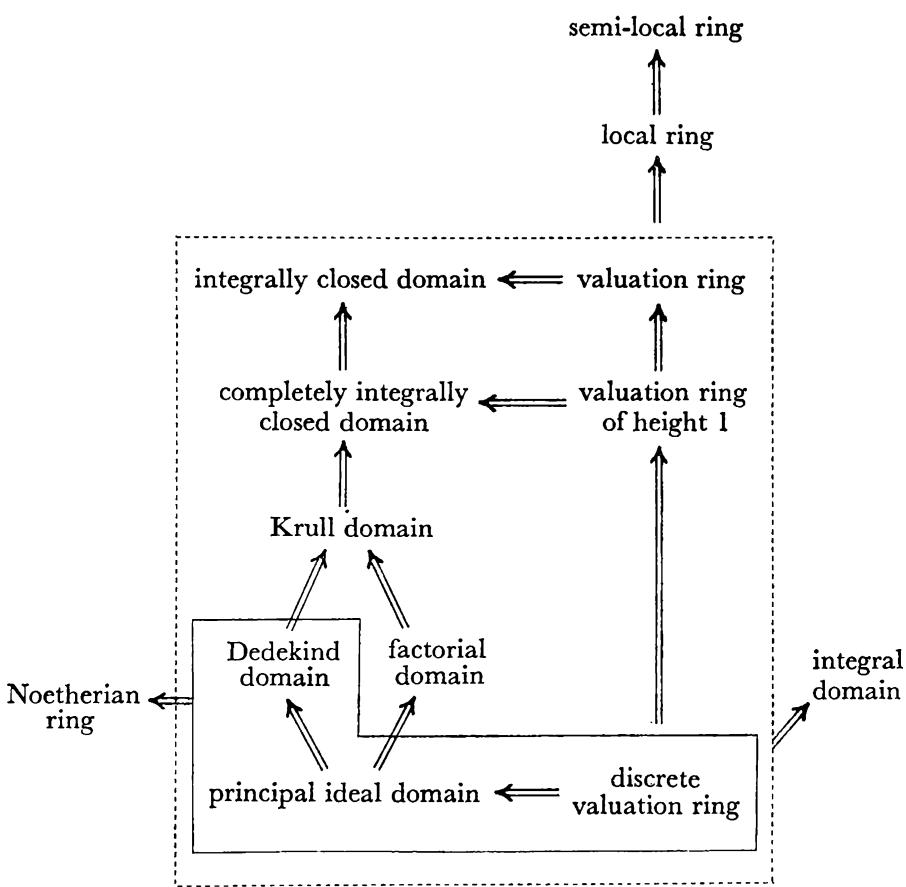
\includegraphics[keepaspectratio]{images/part004_39dc4b31.jpg}}

在 Noether 环的情形下，此表化为下表：

\pandocbounded{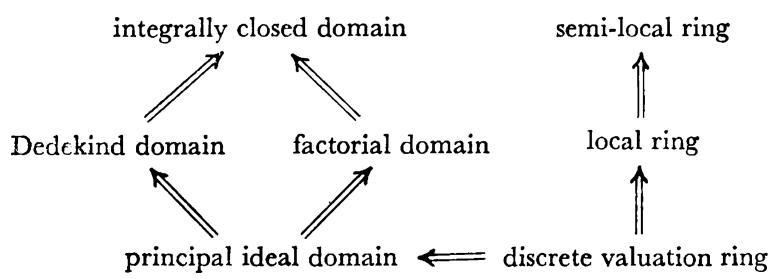
\includegraphics[keepaspectratio]{images/part004_7c195a13.jpg}}

\specialchapter{不变性表 --- I}

在本表及下表中，每一行对应于环可能具有的一个性质，每一列对应于由环 A 导出的一个环（p 表示 A 的一个素理想，S 表示 A 的一个不含 0 的乘性子集，而 A' 表示 A 在 A 的分式域 K 的有限代数扩张 L 中的整闭包）。假定环 A 具有该行所指的性质；本行与某列交叉处的 ``是''（相应地 ``否''、``？''）表示：由该列所指过程从 A 构造的每个环都具有该行所指的性质，这一事实为真（相应地为假、仍未知）。

参考文献指出本书或《代数》一书中证明所述结果的位置；对于下列两部著作中涉及正文或习题未提及的结果，情形同样如此：

\begin{enumerate}
\def\labelenumi{(\arabic{enumi})}
\item
  A. GROTHENDIECK, 代数几何原理，第 IV 章 (Publ. Inst. Htes Études Scient.，第 20 和 24 号，1964)。
\item
  M. NAGATA, 局部环，Interscience (New York)，1962。
\end{enumerate}

A/p

\(S^{-1}A\)

A{[}X{]}

A{[}{[}X{]}{]}

A'

A 为主理想整环

是

是

否 代数 VII, § 1, 习题 1

否

否 代数 VII, § 1, 习题 12

A 为 Dedekind 整环

是

是

否 代数 VII, § 1, 习题 1

否 VII, § 1, 习题 9

是 VII, § 2, 命题 9 的推论 2)

A 为因子分解整环

否 V, § 1, 习题 9

是 VII, § 3, 命题 3

是 VII, § 3, 定理 2

否 VII, § 3, 习题 9

否 代数 VII, § 1, 习题 12

A 为 Noether 整闭整环

否 V, § 1, 习题 9

是 V, § 1, 命题 16 的推论 1

是 V, § 1, 命题 13 的推论 1

是 V, § 1, 命题 14

？（若 L 可分则是；V, § 1, 命题 18 的推论 1）

A 为域或离散赋值环

是 VI, § 3, 第 6 节

是 VI, § 3, 第 6 节

否 代数 VII, § 1, 习题 1

否 VII, § 1, 习题 9

否 V, § 2, 习题 6

A 为域或高度 1 的赋值环

是 VI, § 4

是 VI, § 4, 命题 1

否 代数 VII, § 1, 习题 1

否 VII, § 1, 习题 9

否 V, § 2, 习题 6

A 为赋值环

是 VI, § 1, 定理 1

是 VI, § 1, 定理 1

否 代数 VII, § 1, 习题 1

否 VII, § 1, 习题 9

否 V, § 2, 习题 6

A 为完备赋值环

是 VI, § 5, 命题 1

是 VI, § 7, 命题 3

否 代数 VII, § 1, 习题 1

否 VII, § 1, 习题 9

否 V, § 2, 习题 6

A 为 Krull 整环

否 V, § 1, 习题 9

是 VII, § 1, 命题 6

是 VII, § 1, 命题 13

是 VII, § 1, 习题 9

是 VII, § 1, 命题 12

\specialchapter{不变性表 --- II}

在本表中，a 表示 A 的一个异于 A 的理想，S 表示 A 的一个乘性子集，而 A' 表示 A 的整闭包，并假定它是整环。

A/a

\(S^{-1}A\)

A{[}X{]}

A{[}{[}X{]}{]}

A\textquotesingle{}

A 为局部环

是

否 II, § 2, 命题 11

否

是 代数 IV, § 5, 命题 4

否 V, § 2, 习题 20

A 为局部完备环

？若 A 为 Noether 环则是（III, § 3, 命题 6）

否 II, § 2, 命题 11

否

是 III, § 2, 命题 6

？若 A 为 Noether 环则是（1）

A 为半局部环

是

否 IV, § 2, 习题 23(c)

否

是 代数 IV, § 5, 命题 4

？若 A 为 Noether 环则是 V, § 2, 习题 7

A 为半局部完备环

？若 A 为 Noether 环则是（III, § 3, 命题 6）

否 IV, § 2, 习题 23(c)

否

是 III, § 2, 命题 6

A 为 Noether 环

是 代数 VIII, § 2, 命题 6

是 II, § 2, 命题 10 的推论 2

是 III, § 2, 定理 2 的推论 1

是 III, § 2, 定理 2 的推论 6

否 V, § 1, 习题 21 若 A 局部完备则是（1）A\textquotesingle{} 总是 Krull 整环（2）

\specialchapter{完备化下的不变性}

\begin{enumerate}
\def\labelenumi{(\alph{enumi})}
\tightlist
\item
  设 A 是一个环，m 是 A 的一个异于 A 的理想。赋予 A 以 m-进拓扑，并以 \(\hat{A}\) 表示其 Hausdorff 完备化。
\end{enumerate}

A 为 Hausdorff 环

是

A 为 Noether 环

是（III, § 3, 命题 8）

A 为局部环

是（III, § 2, 命题 19）

A 为半局部环

是（III, § 2, 命题 19 的推论）

A 为 Zariski 环

是（III, § 3, 命题 8）

\textbf{\(\hat{\mathbf{A}}\)}\par

\begin{enumerate}
\def\labelenumi{(\alph{enumi})}
\setcounter{enumi}{1}
\tightlist
\item
  现在设 \(\mathbf{A}\) 是局部 Noether 环，且 \(\mathfrak{m}\) 是其极大理想。
\end{enumerate}

A 为整环

A 为整闭整环

A 为离散赋值环

A 为约化环

\textbf{\(\hat{\mathbf{A}}\)}\par

否（III, § 3, 习题 15 (b)）

对优良环是（1）

%\pandocbounded{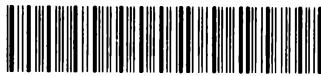
\includegraphics[keepaspectratio]{images/part004_82ba3e9c.jpg}}\\

